% !TeX root = ../thuthesis-example.tex

\chapter{现阶段区块链面临的问题}

本节分为- 5.1 技术限制与挑战,- 5.2 监管和合规性难题,- 5.3 市场认知与接受度问题。由于考虑到本篇是新生向的学术导论,以及受当地区块链政策与法规影响,将重点介绍- 5.1 技术限制与挑战,监管和合规性难题 与 市场认知与接受度问题 将简略带过。

目前讨论的区块链的技术限制与挑战,主要分为安全问题,跨链效率问题和可扩展性问题。

由于这次宣讲的深圳大学区块链实验室的成果主要是区块链应用和区块链安全,因此以 下将从区块链安全展开。根据网络系统的安全需求, 结合区块链的特点, 区块链系统构建的基本安全目标是通过密码学和网络安全等技术手段, 保护区块链系统中的数据安全、共识安全、隐私保护、智能合约安全和内容安全, 各安全目标之间的关系如图 5.1 所示. 

\begin{figure}
	\centering
	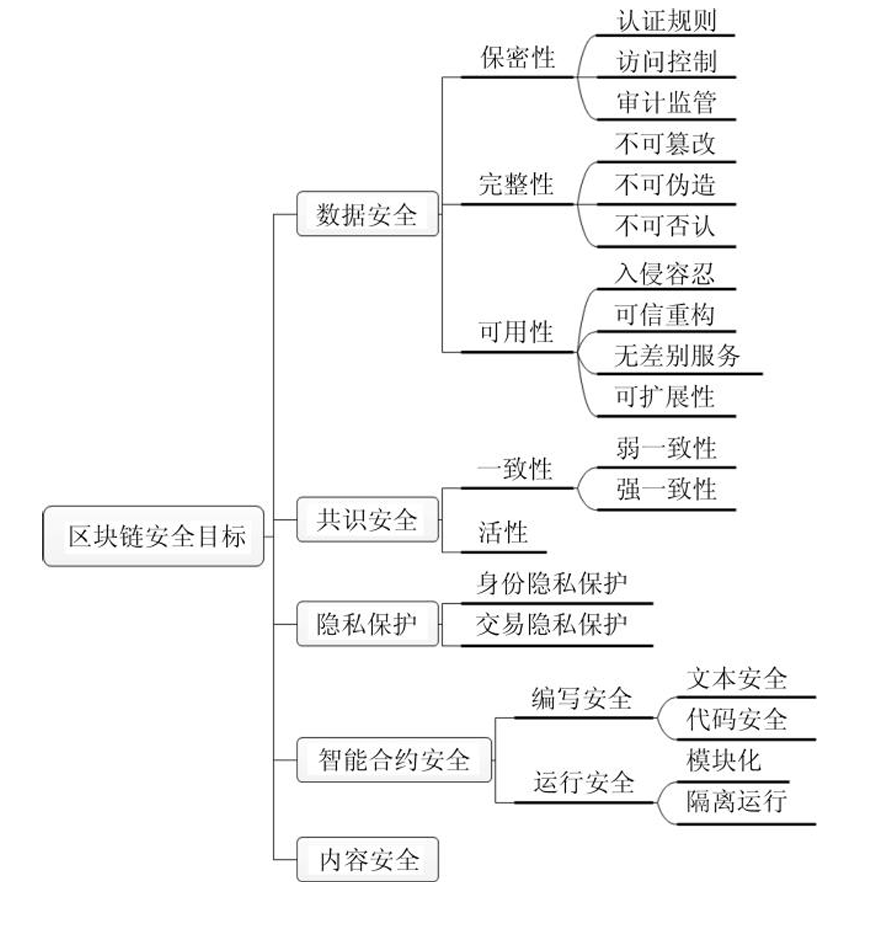
\includegraphics[width=0.5\textwidth]{img/1.png}
	\caption{区块链安全目标}
	\label{fig:example}
\end{figure}

其中, 数据安全是区块链的首要安全目标. 共识安全、智能合约安全、隐私保护和内容安全等安全目标与数据安全联系紧密, 是数据安全目标在区块链各层级中的细化, 也是区块链设计中需要特别考虑的安全要素


section{技术限制与挑战}

为了更好地解释区块链体系结构中提供的安全机制和出现的安全问题, 本文采用《区块链技术发展现状与展望》[6] 中提出的数据层、网络层、共识层、激励层、合约层和应用层六层体系架构, 并以此为基础从信息安全的角度对六层体系架构进行重新解释. 每层可细分为基础模块和安全模块两部分, 如图5.2 所示. 其中, 基础模块是用于实现该层主要功能的基本组件. 安全模块则是用于保障各层安全性, 为上层提供安全稳定技术支持的安全组件。

\begin{figure}
	\centering
	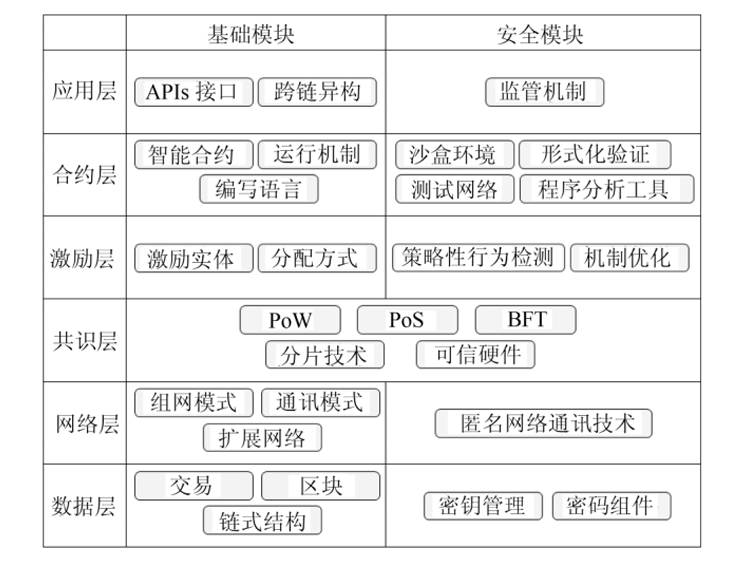
\includegraphics[width=0.5\textwidth]{img/2.png}
	\caption{区块链体系架构}
	\label{fig:example}
\end{figure}

关于区块链的技术限制与挑战,我们使用自底向上方法构建区块链体系架构并阐述每个层级所面临的安全问题。(如同计算机网络的自顶向下方法的七层理论网络) \\


数据层既规定了交易、区块、链式结构在内的狭义区块链的数据结构和存储形式等基本模块, 也包括了关于用户身份、地址的密钥管理机制以及区块链所需的其他密码学组件等安全模块, 是实现其他五层功能的基础. 综合数据层各组件特点, 数据层面临着量子计算威胁、密钥管理不当、交易关联性紧密和密码组件代码漏洞等安全性问题

网络层的核心是确保区块链节点的合法加入和有效通信, 具体包括区块链的组网模式、节点之间的通信模式、扩展网络以及必要的匿名网络通信技术。网络层的安全问题主要包括 P2P 网络的安全问题、网络拓扑被用于攻击以及网络层面的隐私保护问题。

共识层是区块链架构的核心, 主要规定了区块链的共识机制, 确保各节点在网络层提供的网络环境和通信模式中可以共享同一份有效的区块链视图 (View). 区块链的最大创新在于共识层支持的共识机制提供了一种剔除可信第三方的可信数据共享机制, 为上层应用提供安全的账本支持[7]. 

共识层致力于设计高安全性、高效率、低能耗的共识机制, 根据采用的基础协议不同, 可以划分为 5大系列, 包括 PoW、PoS、拜占庭容错协议 (Byzantine fault tolerance, BFT)、分片技术、可信硬件。区块链上的共识机制发展尚不完善, 普遍存在安全性证明不完备、安全性假设不可靠、扩展性差、一致性不稳定、初始化和重构难等问题. 不同类型的共识机制还面临不同的攻击威胁。

激励层需要解决的主要问题是经济学上的激励不相容问题, 具体指参与维护区块链的矿工不会实施危害安全性的恶意攻击, 但是会以自身利益最大化来指导自己的挖矿策略. 这种策略与区块链整体利益形成冲突, 破坏区块链系统效率和稳定性, 包括自私挖矿攻击[8]、Nothing at stake 攻击、扣块攻击 (Withholding attack)[9] 和激励不可持续问题。

合约层由于智能合约代码开源、涉及数字资产转移, 一旦代码漏洞被利用, 会造成不可逆转的损失. 除智能合约创建者在设计业务逻辑时的文本安全问题以外, 合约层还面临智能合约代码漏洞、外部数据源调用、缺乏形式化验证、难实现隐私保护等问题。

区块链在金融、供应链、能源等多领域具有广泛的应用场景(将会在第6节详细叙述). 虽然在不同的应用场景下, 应用层需要反映不同的区块链的业务功能, 在设计上略显差异. 但是, 应用层作为直接与用户交互的区块链层级, 在架构设计上还具有一定的共同点. 一般地, 应用层需要具备 API 接口、跨链异构和监管技术. 从当前区块链应用发展来看, 应用层设计面临跨链操作难、监管技术缺失和应用层攻击等问题.

\begin{figure}
	\centering
	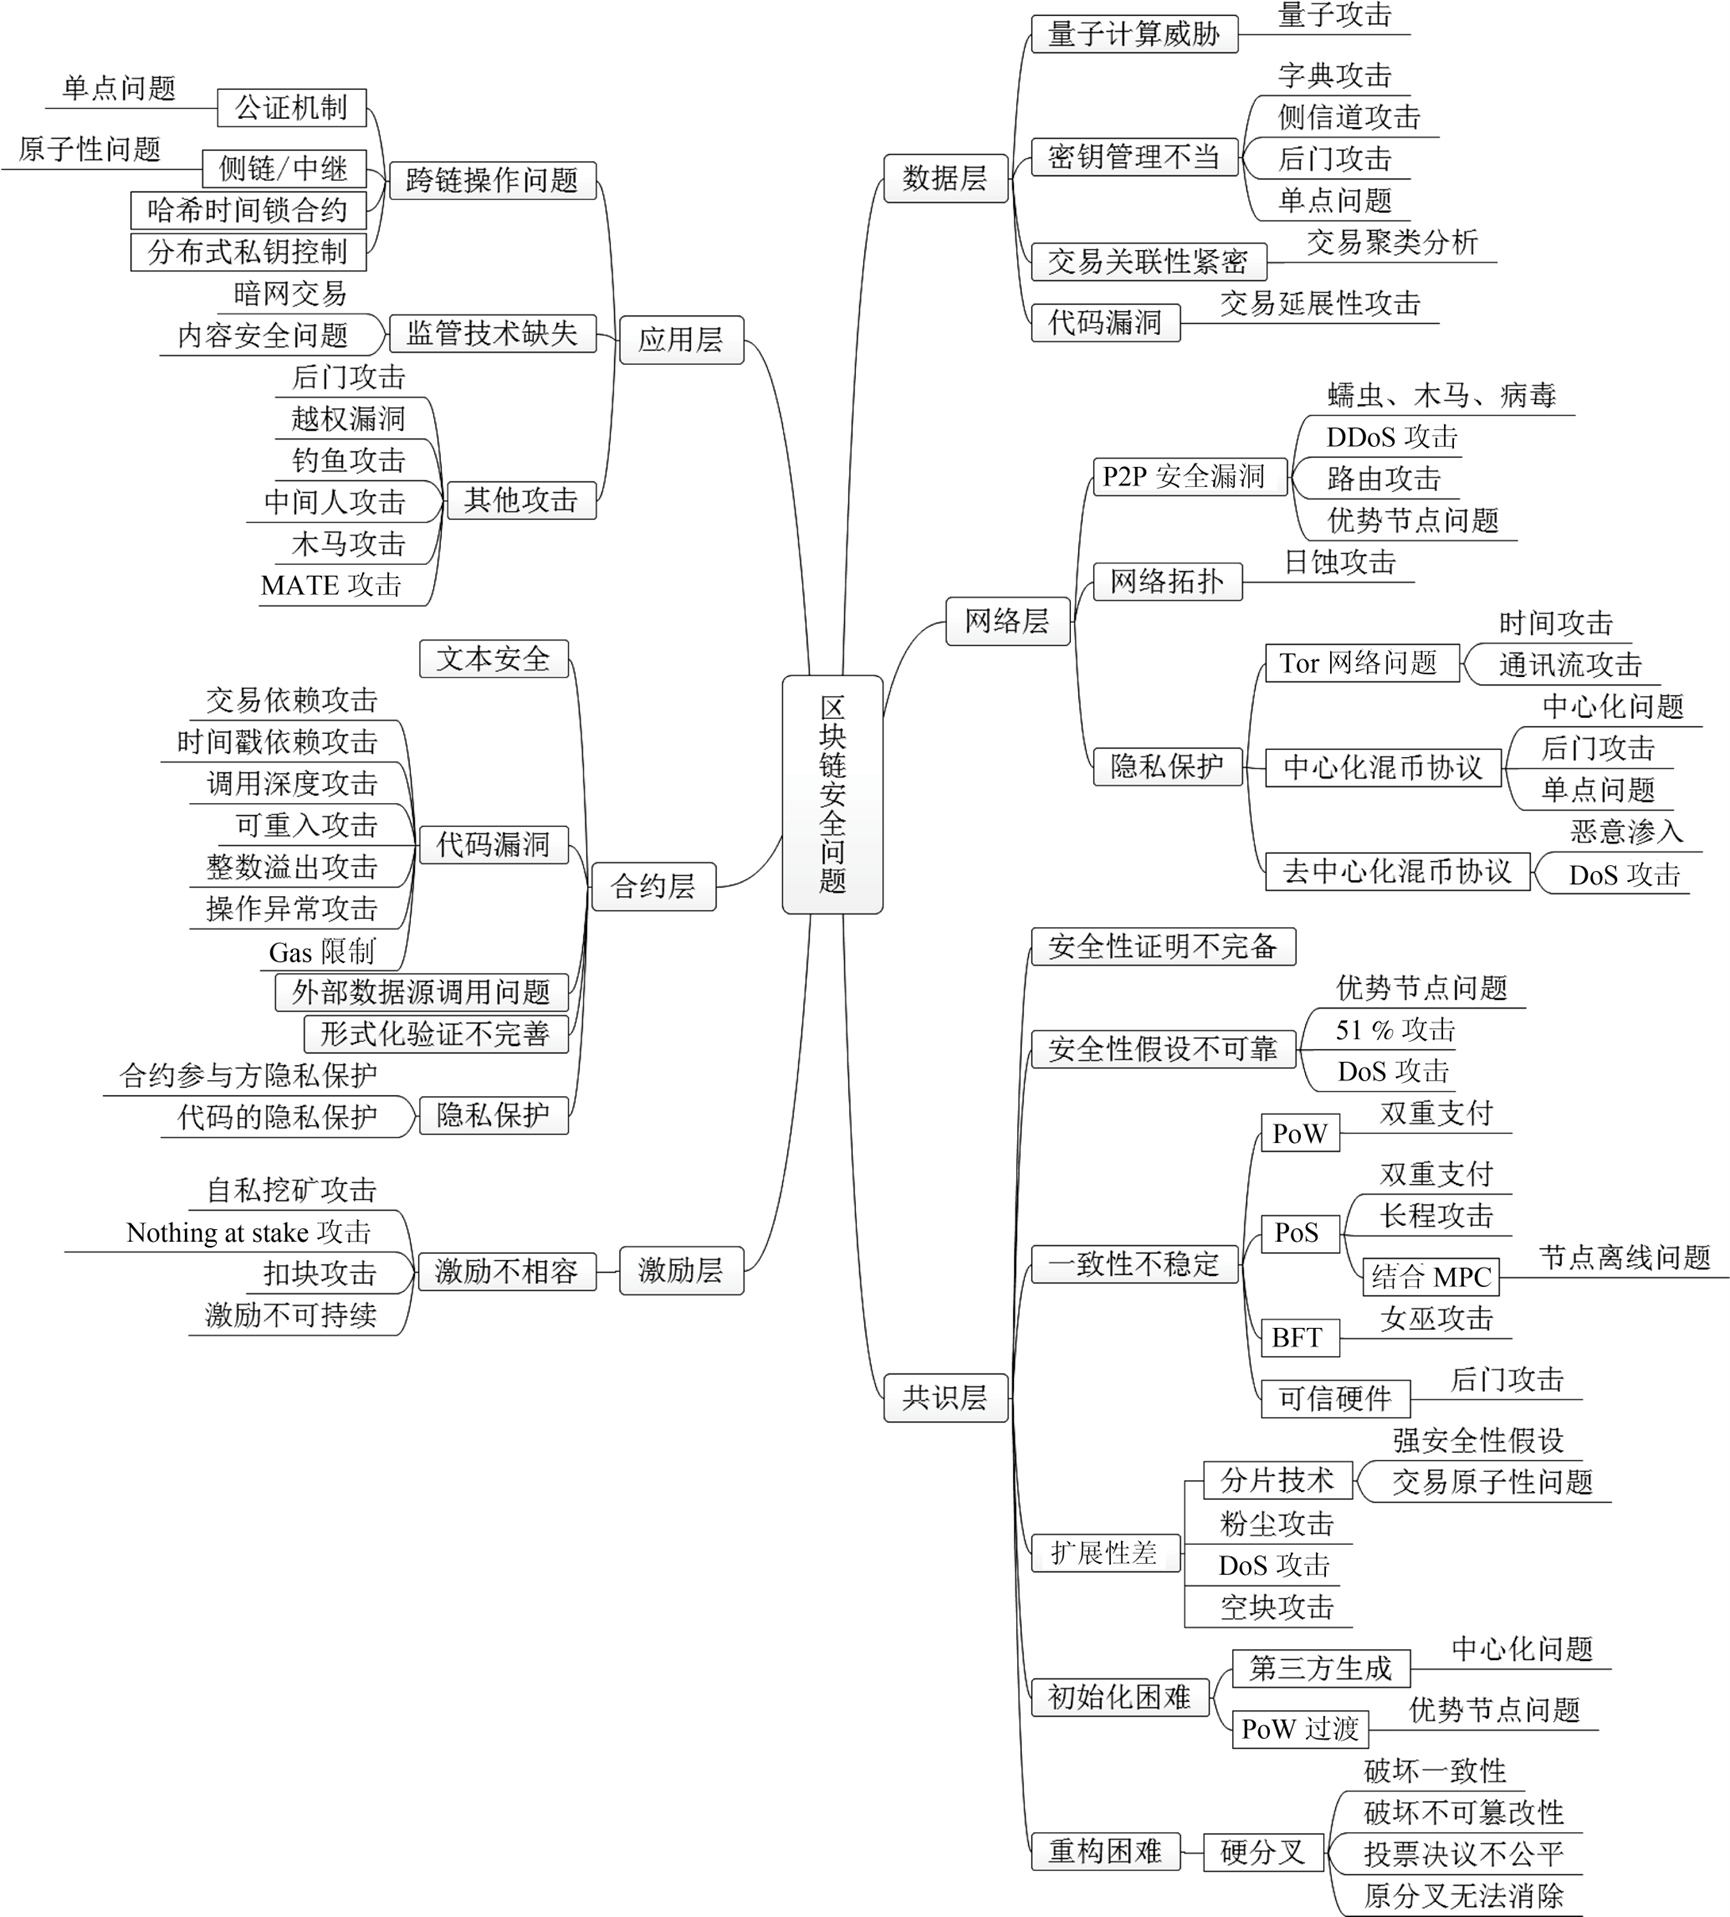
\includegraphics[width=0.5\textwidth]{img/3.png}
	\caption{区块链的安全问题}
	 Fig.3	Security threats on blockchain [10]
	\label{fig:example}
\end{figure}

\section{监管和合规性难题}

由于本小节部分涉及敏感的当地的区块链政策与法律法规,因此使用奥卡姆剃刀原则,抛却本国区块链合规以及跨国区块链监管等跨国政府需要解决的难题,本小节聚焦于作为一个区块链发行商与加密货币拥有者需要解决的监管和合规性难题。 \\

区块链网络作为去中心化的分布式系统, 其各节点在交互过程中不可避免地会存在相互竞争与合作的博弈关系, 这在比特币挖矿过程中尤为明显. 通常来说, 比特币矿池间可以通过相互合作保持各自稳定的收益. 然而, 矿池可以通过称为区块截留攻击 (Block withholding attacks) 的方式、通过伪装为对手矿池的矿工、享受对手矿池的收益但不实际 贡献完整工作量证明来攻击其他矿池, 从而降低对手矿池的收益. 如果矿池相互攻击, 则双方获得的收益均少于不攻击对方的收益. 当矿池收益函数满足特定条件时, 这种攻击和竞争将会造成 “囚徒困境”。 

如何设计合理的惩罚函数来抑制非理性竞争、使得合作成为重复性矿池博弈的稳定均衡 解, 尚需进一步深入研究. 此外, 正如前文提到的, 区块链共识过程本质上是众包过程, 如何设计激励相容的共识机制, 使得去中心化系统中的自利节点能够自发地实施区块数据的验证和记账工作, 并提高 系统内非理性行为的成本以抑制安全性攻击和威胁, 是区块链有待解决的重要科学问题


\section{市场认知与接受度问题}

在中心化社会系统中, 数据通常掌握在政府和大型企业等 “少数人” 手中, 为少数人 “说话”, 其公正性、权威性甚至安全性可能都无法保证.区块链数据则通过高度冗余的分布式节点存储, 掌握在 “所有人” 手中, 能够做到真正的 “数据民主”.就信用基础而言, 中心化社会系统因其高度工程复杂性和社会复杂性而不可避免地会存在 “默顿系统”的特性, 即不确定性、多样性和复杂性, 社会系统中的中心机构和规则制定者可能会因个体利益而出现失信行为;

区块链是实现 CPSS [社会物理信息系统 (Cyber-physical-social systems, CPSS)]平行社会的基础架构之一,其主要贡献是为分布式社会系统和分布式人工智能研究提供了一套行之有效的去中心化的数据结构、交互机制和计算模式, 并为实现平行社会奠定了坚实的数据基础和信用基础。 \\

区块链其核心优势——去除中介和提升透明度——可能对一些传统机构的利益构成威胁。银行、保险公司等中介型机构可能会因为区块链技术的普及而失去市场份额,这导致了这些机构可能对区块链技术的推广持保守甚至抵制的态度。这种市场力量的不平衡,加剧了区块链技术在实践中的推广难度。

除此以外,在民主社会,如何处理和保障对CPSS平行社会抱有敌意的人群(这是的确存在的)的接受度和人权也是一个巨大的问题,毕竟我们不应该使用强制手段去达到一个社会目的,即使它是好的。

